The following Sections describe the methods used in the course of this thesis.

\subsection{Implementation Details}\label{subsec:implementation-details}

All models were implemented with Keras\footnote{\href{https://keras.io/}{https://keras.io/}, last access: 07/01/2020} in Version 2.2.4 using the TensorFlow\footnote{\href{https://www.tensorflow.org/}{https://www.tensorflow.org/}, last access: 07/01/2020} backend in Version 1.15..
The models were trained on Tesla V100-DGXS GPUs with 16GB of RAM.
The model code can be found under \href{https://github.com/LeoIV/master-thesis-leonard}{https://github.com/LeoIV/master-thesis-leonard}.

\subsection{Datasets}\label{subsec:datasets}

Five different datasets were used to train the models.
Four of the datasets contain images of different sizes, the fifth dataset provides additional labels for \textsc{Mnist}.
The images were resized to match the model's excepted input sizes using Lanczos interpolation~\citep[pp. 223, ff]{burger2009principles}.

\subsubsection{CelebA}\label{subsubsec:celeba_dataset}

\begin{wrapfigure}[14]{R}{0.3\textwidth}
    \begin{center}
        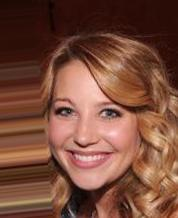
\includegraphics[width=0.28\textwidth]{images/celeba_sample_63.jpg}
    \end{center}
    \caption[CelebA dataset sample image]{A sample image from the CelebA dataset.}
    \label{fig:celeba_sample}
\end{wrapfigure}

The \textit{CelebA} dataset~\citep{liu2015faceattributes} consists of 202,599 RGB images of size 178 x 218 pixels representing celebrities, as well as 40 binary attributes.
The images belong to 10.177 unique identities\footnote{The identities are not revealed.} as well as five \say{landmark annotations}.
They are aligned and cropped resulting in images of same size always showing only one face (see Figure~\ref{fig:celeba_sample} for an example).
The landmark annotations give the positions of facial attributes in the image, specifically of the left and right eye, the nose, and the left and right corner of the mouth.
The binary attributes indicate if the image has certain attributes, for example if the person wears eyeglasses, has black hair, is smiling, etc\footnote{See \href{https://www.kaggle.com/jessicali9530/celeba-dataset\#list\_attr\_celeba.csv}{https://www.kaggle.com/jessicali9530/celeba-dataset\#list\_attr\_celeba.csv} for a complete list of the attributes, login required. Last access: 12/02/2020.}.

\subsubsection{ImageNet}\label{ssec:imagenet}

ImageNet\footnote{\href{http://image-net.org/}{http://image-net.org/}, last access: 12/02/2020.} is a large-scale \say{image database organized according to the WordNet hierarchy}~\citep{imagenet_cvpr09} consisting of over 14 million images as of February 2020.
Accordingly to WordNet\footnote{See \href{https://wordnet.princeton.edu/}{https://wordnet.princeton.edu/}, last access: 12/02/2020.}, on different levels of granularity, the images are subdivided into groups called \say{synsets}~\citep{imagenet_cvpr09}.
For example, the group \textit{woman, adult female} is subordinated to \textit{person, individual, someone, somebody, mortal, soul} and is further subdivided into groups like \textit{old woman} or \textit{lady} \footnote{ImageNet 2011 Fall Release, \href{http://image-net.org/explore}{http://image-net.org/explore}, last access: 12/02/2020.}

A smaller version of ImageNet, commonly called \textit{ILSVRC2012} has been used for \ac{ILSVRC2017}~\citep{ILSVRC15}, consisting of approximately 1,3 million images from 1000 different classes, that were selected, such that \say{there is no overlap between synsets: for any synsets $i$ and $j$, $i$ is not an ancestor of $j$ in the ImageNet hierarchy}~\citep{imagenet_cvpr09}.

This curated version is commonly used as a baseline (\textbf{refs}).

\subsubsection{MNIST}\label{subsubsec:mnist}

\begin{wrapfigure}[9]{R}{0.2\textwidth}
    \begin{center}
        
\includegraphics[width=0.18\textwidth]{images/mnist_sample.png}
    \end{center}
    \caption[MNIST dataset sample image]{A sample image from the MNIST dataset.}
    \label{fig:mnist_sample}
\end{wrapfigure}

MNIST\footnote{\href{http://yann.lecun.com/exdb/mnist/}{http://yann.lecun.com/exdb/mnist/}, last access: 23/04/2020}~\citep{lecun1998gradient} is a widely-used dataset of hand-written digits.
The data is subdivided into a training set of 60.000 images and a test set containing 10.000 images.
The digits are \say{size-normalized and centered}.
The samples are grayscale images of size $28\times 28$pixels.

\subsubsection{Morpho-MNIST}\label{subsubsec:morphomnist}

\begin{figure}
    \centering
    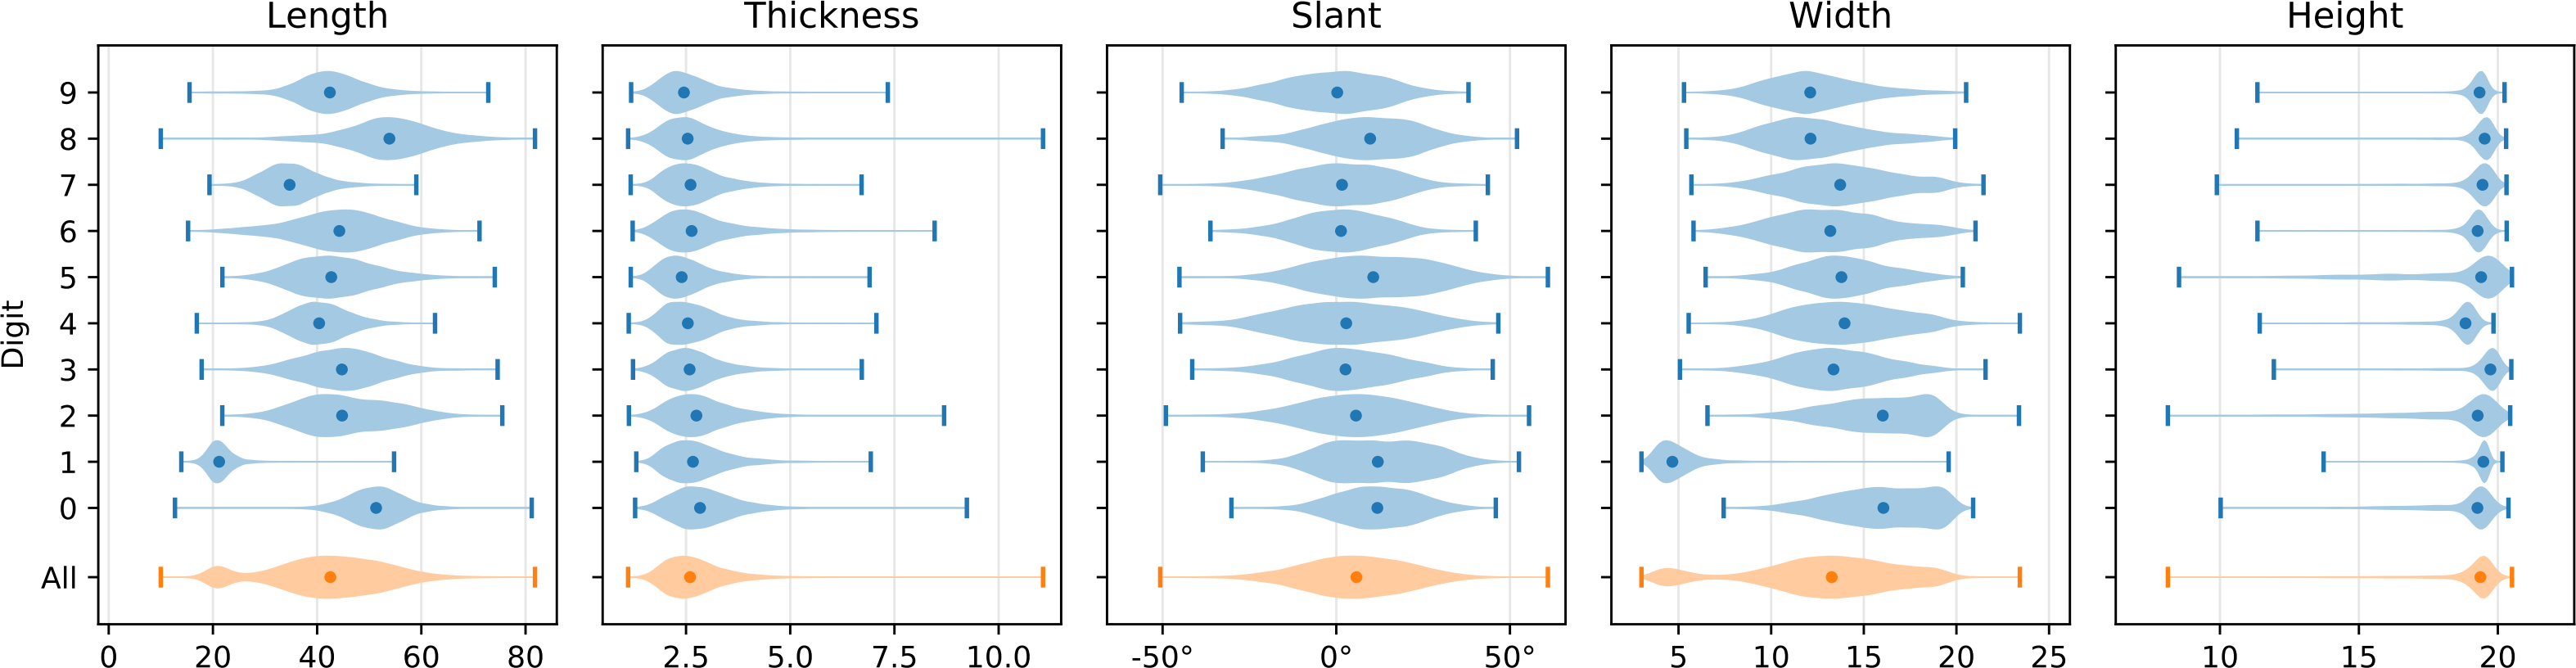
\includegraphics[width=\textwidth]{images/morpho_mnist_distribution.png}
    \caption[Morpho-\textsc{Mnist} distribution]{Distribution of the Morpho-\textsc{Mnist} attributes for the different digits. Taken from~\citep{castro2019morpho}.}
    \label{fig:morpho_mnist_distribution}
\end{figure}

Morpho-\textsc{Mnist}~\citep{castro2019morpho} is an extension of the \textsc{Mnist} dataset that addresses the question: \say{[T]o what extent has my model learned to represent specific factors of
variation in the data?} ~\citep{castro2019morpho}.
To address this questions, Morpho-MNIST provides the following (continuous) labels of morphological attributes of the MNIST samples: stroke length, stroke thickness, slant, width, and height.

Besides providing additional labels of low-level MNIST attributes, Morpho-MNIST provides a toolbox to measure (i.e~ calculate the morphological labels) and perturb MNIST images.
The perturbation toolbox allows it to thin, thicken, swell, and to add fractures to an image.
Morpho-MNIST also provides pre-computed datasets that were built using the perturbation toolbox.

Importantly, the distribution of the morphological attributes partly is highly skewed (for example Thickness and Height, see Figure~\ref{fig:morpho_mnist_distribution}).

\subsubsection{dSprites}
dSprites\footnote{\href{https://github.com/deepmind/dsprites-dataset/}{https://github.com/deepmind/dsprites-dataset/}, last access: 5/28/2020}~\citep{dsprites17} is a dataset designed \say{to assess the disentanglement properties of unsupervised learning methods.}
It contains 737,280 grayscale images of size $64\times 64$ pixels.
The images were generated from \say{6 ground truth independent latent factors}: color, shape, scale, orientation, $x$-position, and $y$-position.
The color is white in all images.
The shapes are: square, ellipse, and heart.
For the other factors, points are chosen evenly along their support: six values in $[0.5, 1]$ (scale), 40 values in $[0, 2\pi]$ (orientation), 32 values in $[0, 1]$ ($x$-position and $y$-position).
Each factor combination only occurs once in the data set.

The dataset also contains the factor labels for each image.

\subsection{Models}\label{subsec:models}

Four different base \ac{VAE} models were evaluated in the course of this thesis.
Furthermore, two \say{AlexNet} models were used for some additional experiments.

The models are described in the following.
Importantly, the models were varied based on the input dimensionality, are more detailed description can be found in Appendix~\textbf{REF}.

\subsubsection{VAE Model}

\begin{figure}
    \centering
    \begin{subfigure}{.5\textwidth}
        \centering
        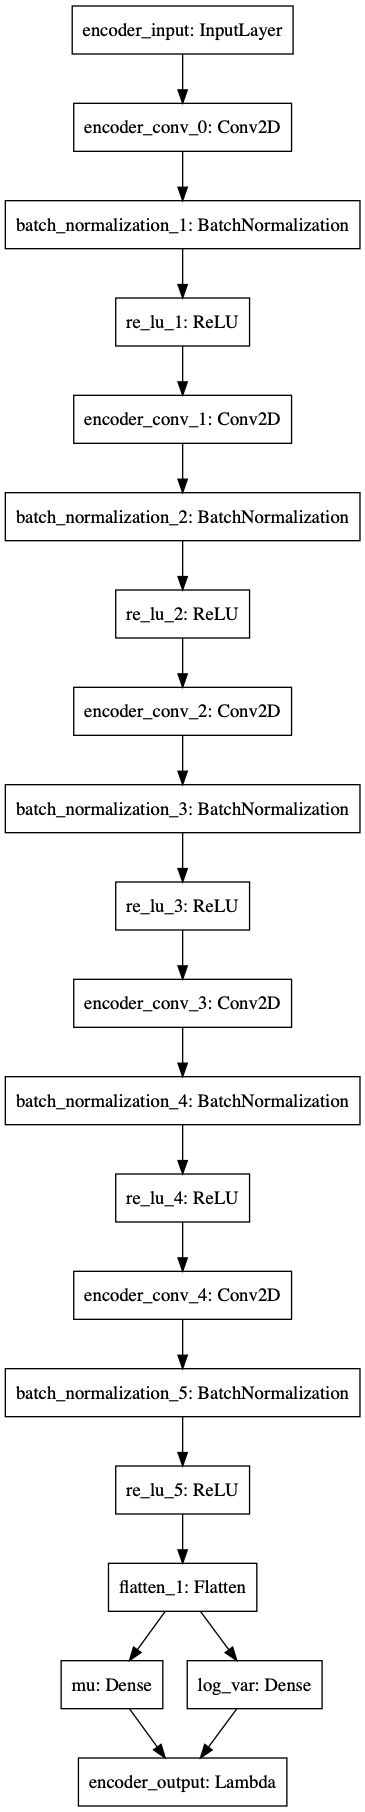
\includegraphics[width=\textwidth,height=.85\textheight,keepaspectratio]{images/vae/encoder.png}
        \caption{Encoder}
    \end{subfigure}%
    \begin{subfigure}{.5\textwidth}
        \centering
        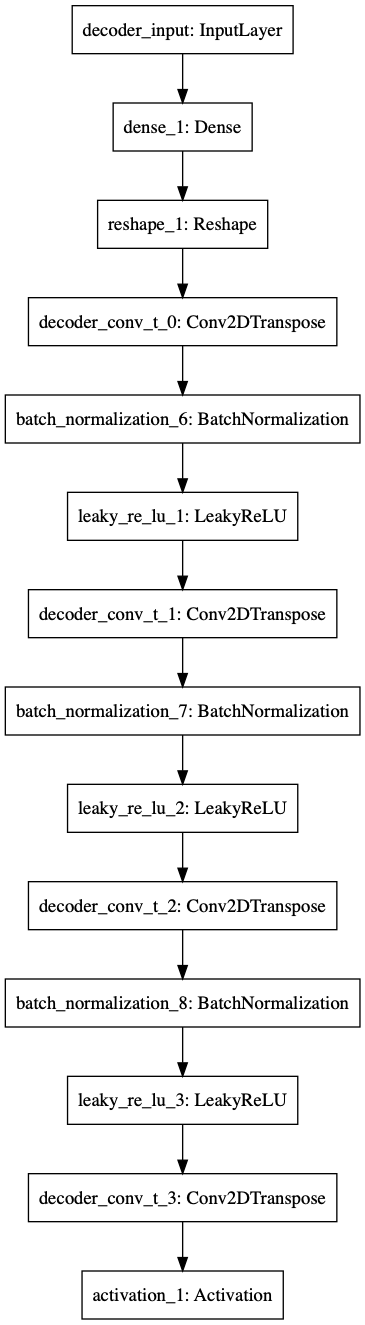
\includegraphics[width=\textwidth,height=.85\textheight,keepaspectratio]{images/vae/decoder.png}
        \caption{Decoder}
    \end{subfigure}
    \caption{\ac{VAE} model structure}
    \label{fig:vae_model_structure}
\end{figure}

The \ac{VAE} model (see Section-\ref{fig:vae_model_structure}) consists of an encoder and a decoder.
The encoder is made up of multiple \say{Convolution, Activation, Batch-Normalization}-blocks, followed by the embedding layer.
The embedding layer predicts $\mu$ and $\log \sigma^2$ and performs the resampling by:
\begin{align}
    z &= \mu + \epsilon\sigma \\
    \epsilon &\sim \mathcal{N}(0, \bm{I}).
\end{align}
The encoder input size is equal to the decoder output size and varies with the experiment.
Also, the number of \say{Convolution, Activation, Batch-Normalization}-blocks is chosen depending on the input size, as smaller input sizes require fewer layers to achieve a receptive field of the input size.
The batch-normalization~~\citep[pp. 317, ff.]{Goodfellow-et-al-2016} can be omitted\footnote{It is stated in the experiments if batch-normalization is omitted.}/
The activation can be either ReLU~\citep[p. 173]{Goodfellow-et-al-2016} or LeakyReLU~\citep[p. 192]{Goodfellow-et-al-2016} and is ReLU unless stated otherwise.
The convolutions use zero-padding unless stated otherwise.
Encoder and decoder use stridden convolutions for downsampling unless stated otherwise.

The decoder uses similar blocks as the encoder but employs transposed convolutions~\citep[pp. 356, ff.]{Goodfellow-et-al-2016} instead of convolutions to upsample feature maps.
The output layer of the decoder uses a sigmoid activation instead of ReLU.

\subsubsection{VLAE Model}

\begin{figure}
    \centering
    \begin{subfigure}{.5\textwidth}
        \centering
        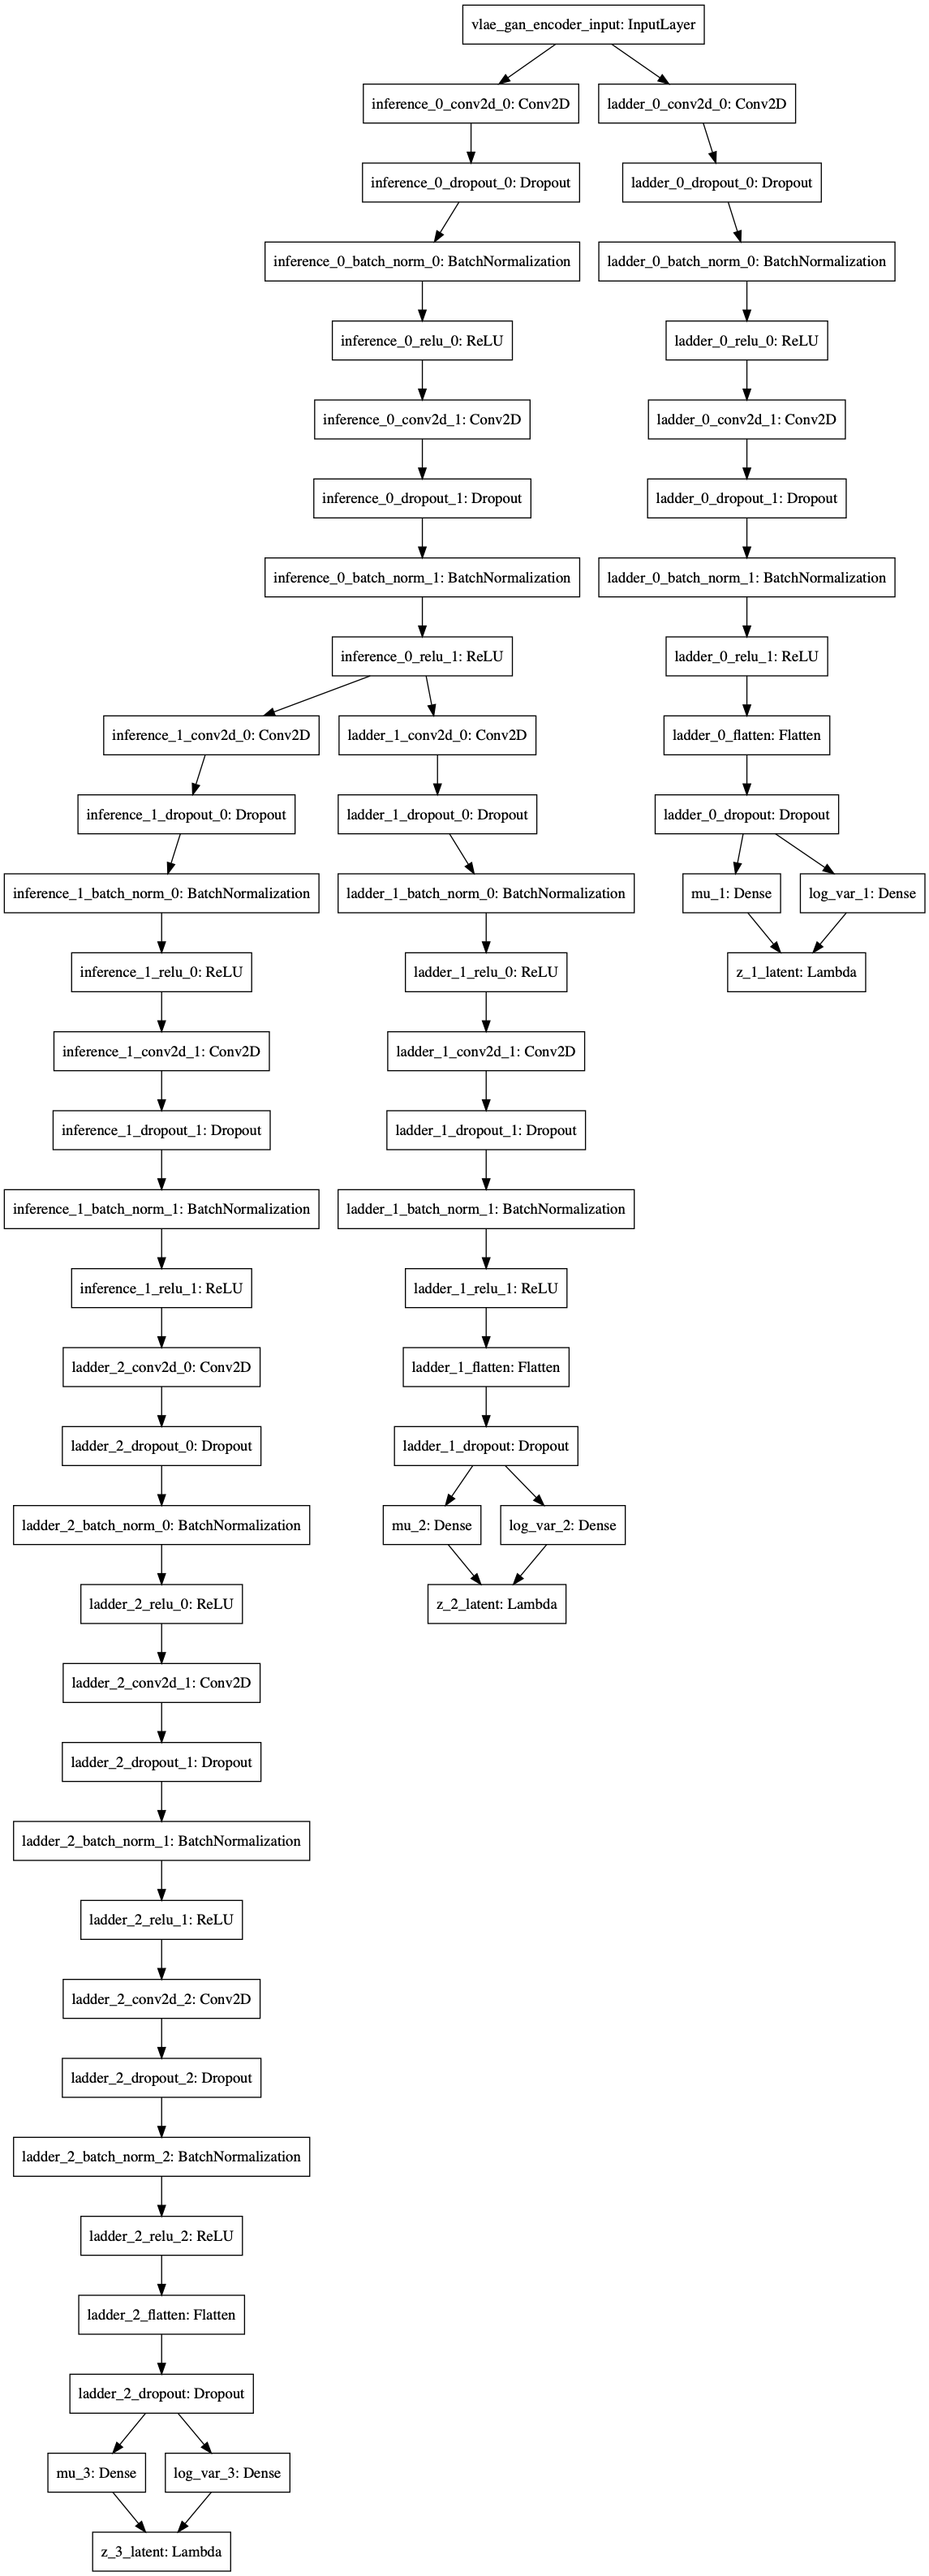
\includegraphics[width=\textwidth,height=.85\textheight,keepaspectratio]{images/vlae/encoder.png}
        \caption{Encoder}
    \end{subfigure}%
    \begin{subfigure}{.5\textwidth}
        \centering
        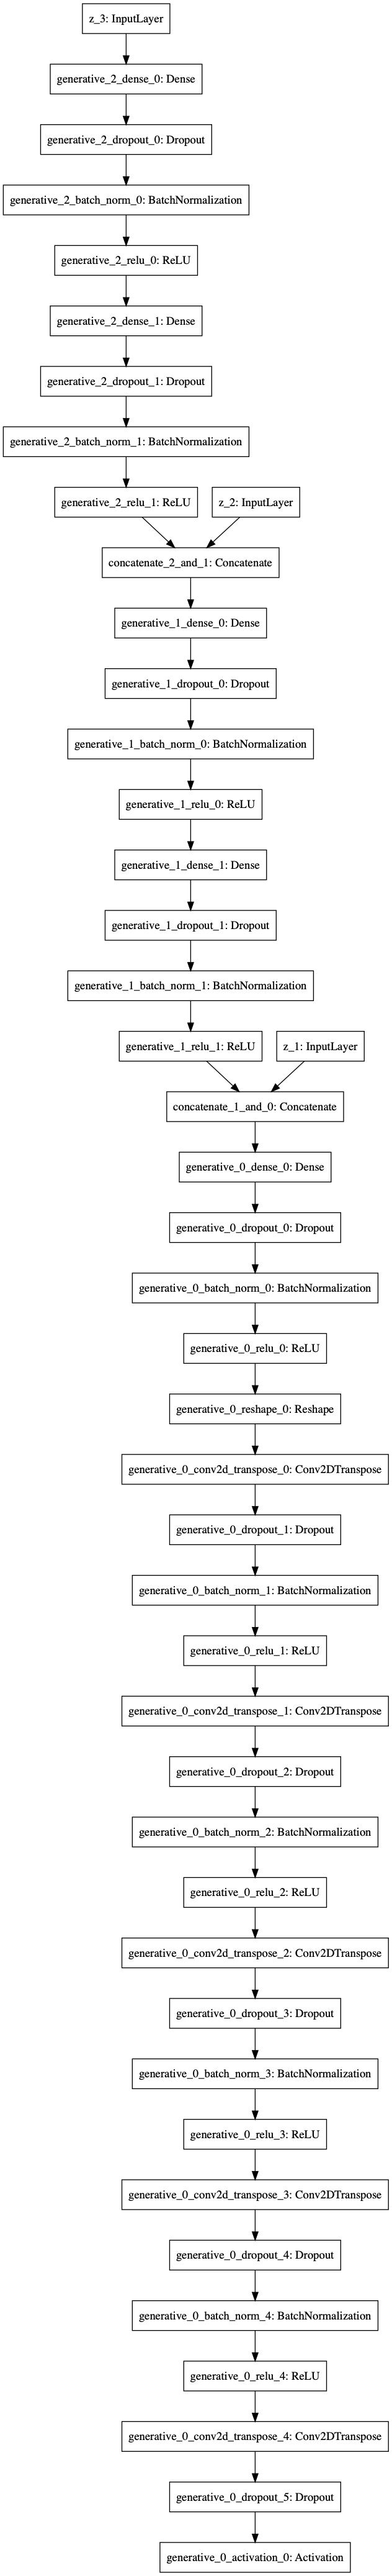
\includegraphics[width=\textwidth,height=.85\textheight,keepaspectratio]{images/vlae/decoder.png}
        \caption{Decoder}
    \end{subfigure}
    \caption{\ac{VLAE} model structure}
    \label{fig:vlae_model_structure}
\end{figure}

\subsubsection{VAE-GAN Model}

\subsubsection{VLAE-GAN Model}

\subsubsection{AlexNet Classifier}

\subsubsection{AlexNet VAE}


%\subsection{Visual Features Variational Autoencoders}\label{subsec:visual-features-variational-autoencoders}
%Different questions were asked investigate whether \acp{VAE} are a biologically plausible model of the Visual Cortex.

%One essential prerequisite is the emergence of Gabor wavelets (\textbf{Ref}).
%As discussed in Section~\ref{subsec:visual_features_in_neural_networks}, Gabor wavelets do emerge in deep convolutional networks, trained on image classification~\citep{krizhevsky2012imagenet} (\textbf{Ref: at least one more paper }), specifically on the ImageNet dataset (\textbf{ref}).\par
%The following approaches were taken to see if Gabor wavelets do naturally emerge in \acp{VAE} (\textbf{explain \say{naturally}}).\par
%First, the convolutional kernels in a \ac{VAE} that was sucessfully trained on the CelebA (\textbf{ref}) dataset in terms of image reconstruction were examined in terms of emergence of Gabor wavelets (\textbf{explain network architecture}).
%Subsequently, the size of the convolutional kernels in the first layer was increased to size 11x11 \footnote{This is the same kernel size of the first layers used in~\citet{krizhevsky2012imagenet}.} as they were too small to successfully represent any Gabor wavelets~\citep{han2019variational}.
%Since still no Gabor wavelets emerged (see Section~\ref{subsec:results_visual_features_in_variational_autoencoders}), the question was raised whether this was because of the different network architectures of AlexNet and the \say{CelebA VAE}, or the dataset, or both.

%\begin{figure}
%    \centering
%    \begin{subfigure}{.5\textwidth}
%        \centering
%        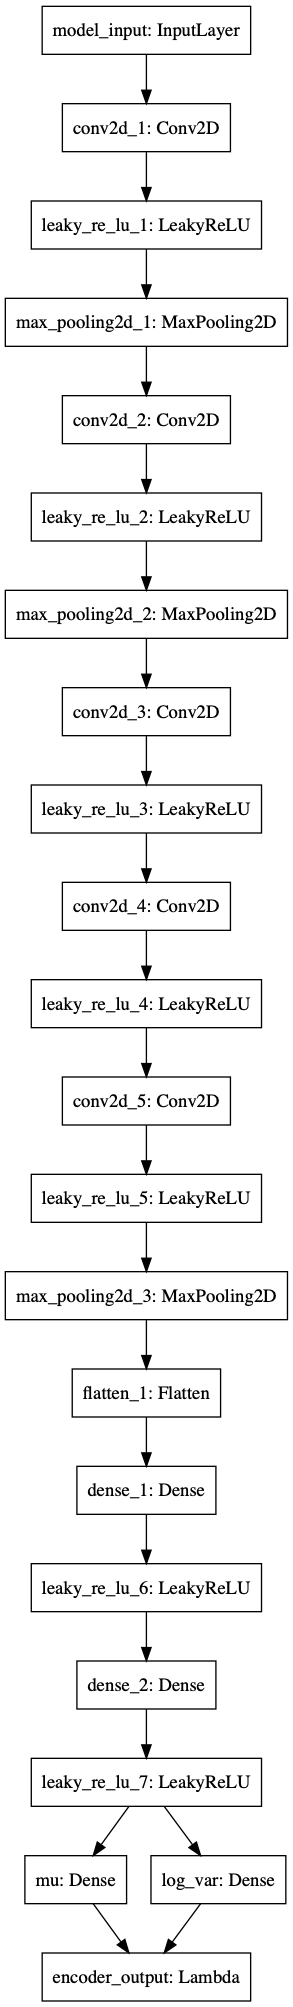
\includegraphics[width=\textwidth,height=.9\textheight,keepaspectratio]{images/alexnet-vae/encoder.png}
%        \caption{Encoder}
%    \end{subfigure}%
%    \begin{subfigure}{.5\textwidth}
%        \centering
%        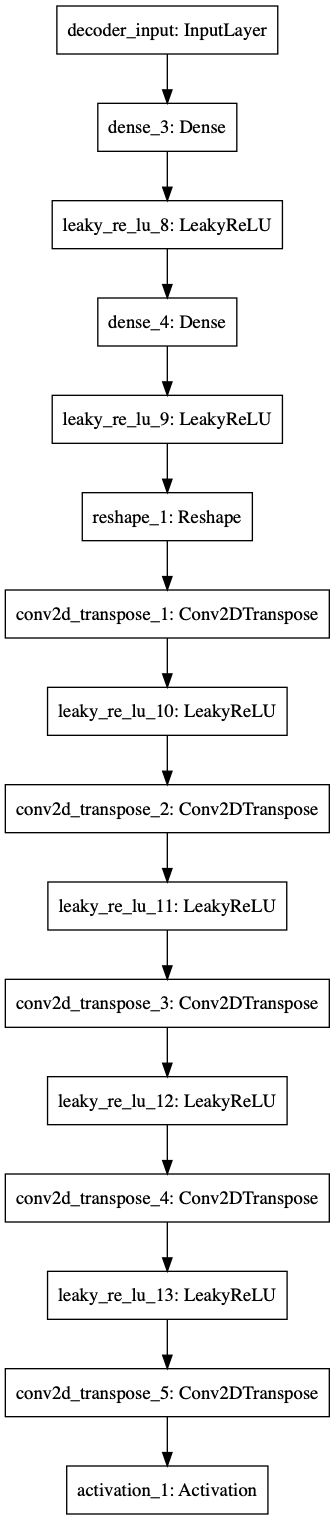
\includegraphics[width=\textwidth,height=.9\textheight,keepaspectratio]{images/alexnet-vae/decoder.png}
%        \caption{Decoder}
%    \end{subfigure}
%    \caption{AlexNet-VAE Network}
%    \label{fig:alexnet-vae-encoder}
%\end{figure}
%
%To further localize the so-far cause for the non-existence of Gabor wavelets, an \say{AlexNet-like-VAE} (subsequently called AlexNet-VAE, see Figure~\ref{fig:alexnet-vae-encoder}) was trained on ImageNet.
%This \ac{VAE} consists of an encoder part that closely resembles AlexNet.
%The output-layer, however, was changed in terms of size and activation function.
%First of all, the output size was allowed to be dynamical to allow different embedding sizes, i.e.\ differently sized multivariate Gaussians.
%Also, the activation function was changed from Softmax (\textbf{ref}) to \ac{LeakyReLU} (\textbf{ref}).
%Furthermore, all other activations were also changed to \ac{LeakyReLU} due to its advantages over \ac{ReLU} (\textbf{which ones? explain}).
%The encoder is was followed by the reparametrization layer and, subsequently, the decoder part which basically consists of the inverse AlexNet structure.\par
%
%\begin{figure}
%    \centering
%    \begin{center}
%        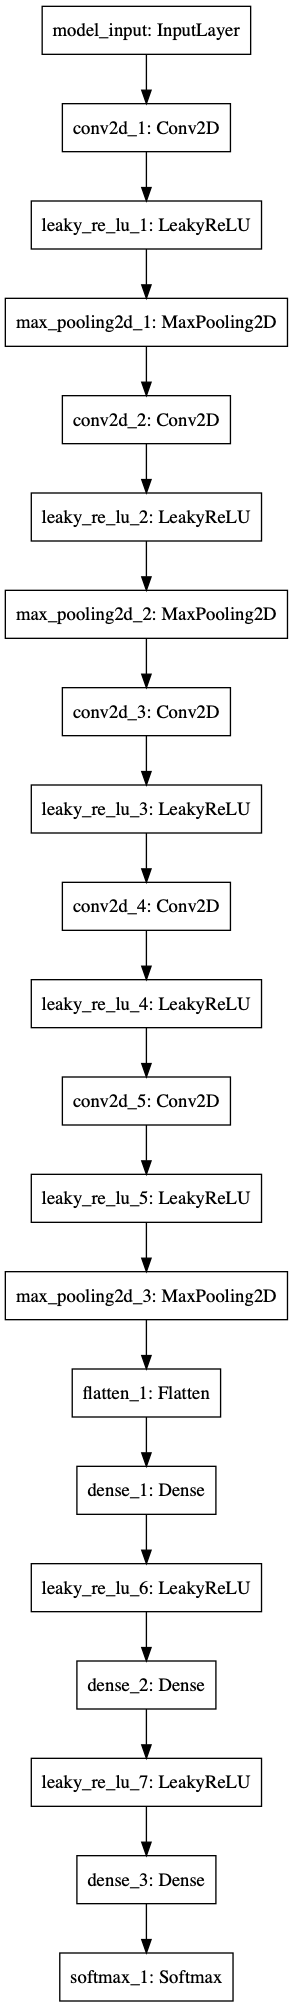
\includegraphics[height=0.9\textheight]{images/alexnet/model.png}
%    \end{center}
%    \caption[AlexNet Network]{AlexNet-inspired Image Classification Network}
%    \label{fig:alexnet}
%\end{figure}
%
%To cross-check the results of the AlexNet-VAE, only the encoder part was trained on ImageNet and image classification, using the Softmax activation in the last layer but keeping the \ac{LeakyReLU} activations in all other layers (see Figure~\ref{fig:alexnet}).
%
%As it turned out that also in the AlexNet-VAE no Gabor wavelets emerged (see Section~\ref{subsec:results_visual_features_in_variational_autoencoders}), the image classification AlexNet-like network was used as an encoder with frozen weights and only the decoder part was trained to see if using a network trained on image classification has certain disadvantages when being used as a decoder in a \ac{VAE} compared to a decoder trained from scratch.

